\section{Kollaborative Robotik}
Menschen und Roboter teilen sich den selben Arbeitsraum.
Die Wiederholgenauigkeit und Ausdauern von Robotern sollen mit den individuellen Fähigkeiten von Menschen kombiniert werden.\newline
\begin{minipage}{0.49\linewidth}
\begin{itemize}
    \item Sicherheit
    \begin{itemize}
        \item Ohne Schutzeinrichtung
        \begin{itemize}
            \item weniger platz
            \item mobil
        \end{itemize}
        \item Kraft-Drehmomentsensorik
        \item Reduzierte Geschwindigkeit   
    \end{itemize}
    \item Eigenschaften
    \begin{itemize}
        \item[+] Platzsparend
        \item[+] bezahlbar
        \item[+] felxibel
        \item[+] Kraftempfindlichkeit
        \item[-] Langsam
    \end{itemize}
    \item Applikation
    \begin{itemize}
        \item Qualtitätskontrolle
        \item Montage (3te-Hand)
        \item Handling
    \end{itemize}
\end{itemize}
\end{minipage}
\begin{minipage}{0.5\linewidth}
    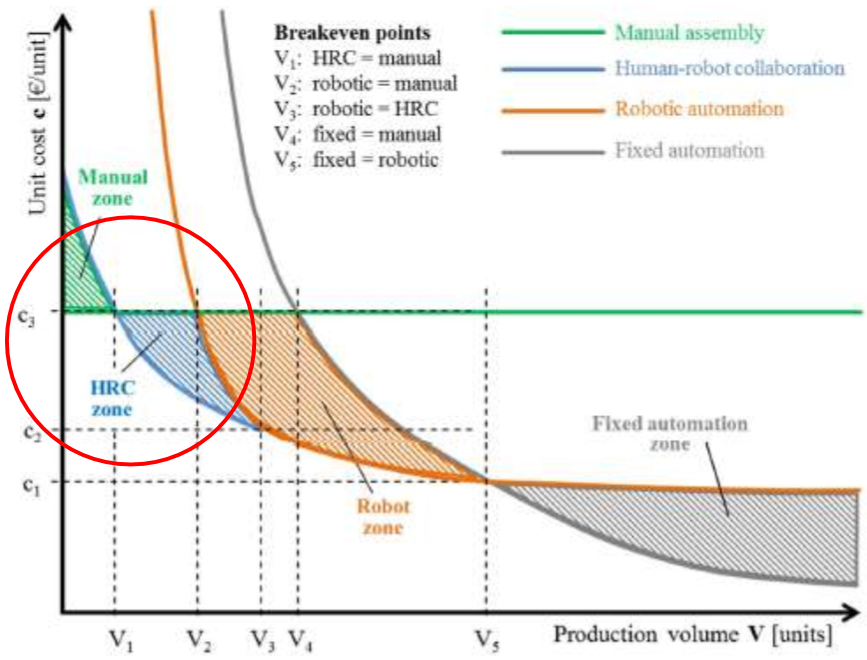
\includegraphics[width=\linewidth]{./bilder/wirtschaft}
\end{minipage}
\subsection{MRK-Schutzarten}
\begin{minipage}{\linewidth}
    \subsubsection{Sicherer Halt}
    \begin{minipage}{0.7\linewidth}
    \textbf{Methode 1}\newline
    \begin{tabular}{p{2.2cm} p{10cm}}
        \textbf{Prinzip}&
        Roboterbewegung wird angehalten bevor eine Person den Kollaborationsraum betritt
        \\
        \textbf{Betriebsweise}&
        Wenn die Sicherheitsüberwachung aktiv und die Roboterbewegungn angehalten ist,
        ist es dem Bedienpersonal erlaubt, den Kollaborationsraum zu betretten.
        Das Robotersystem startet erst wider nach dme Verlassen des Personals aus dem Kollaborationsbereich.
        \\
        \textbf{Anwendungs -bereich}&
        Be- und Entladen \newline
        Kontrollieren der Werkstücke
        \\
    \end{tabular}
    \end{minipage}
    \begin{minipage}{0.3\linewidth}
    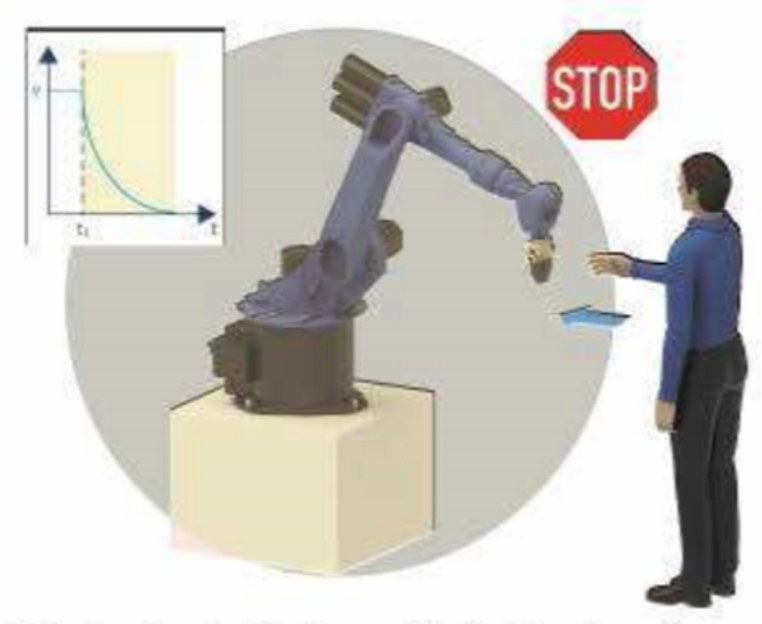
\includegraphics[width=\linewidth]{./bilder/SchutzMRKm1}
    \end{minipage}
\end{minipage}

\begin{minipage}{\linewidth}
    \subsubsection{Handführung}
    \begin{minipage}{0.7\linewidth}
    \textbf{Methode 2}\newline
    \begin{tabular}{p{2.2cm} p{10cm}}
        \textbf{Prinzip}&
        Roboterbewegung wird vom Mitarbeiter aktiv mit geeigneter Ausrüstung gesteuert.
        \\
        \textbf{Betriebsweise}&
        Bevor die Bedienperson den Kollaborationsraum betreten darf, führt das Robotersystem einen überwachten Halt aus.
        Die Aufgabe wird durch manuelle Betätigung der Führungseinrichtung, die sich am Endeffektor des Roboters oder dessen nähe befindet, ausgeführt.
        \\
        \textbf{Anwendungs- bereich}&
        Handgeführte Montagen, Lackieren\newline
        Roboter als Montage-Tool\newline
        Produktion mit kleiner Stückzahl
        \\
    \end{tabular}
    \end{minipage}
    \begin{minipage}{0.3\linewidth}
    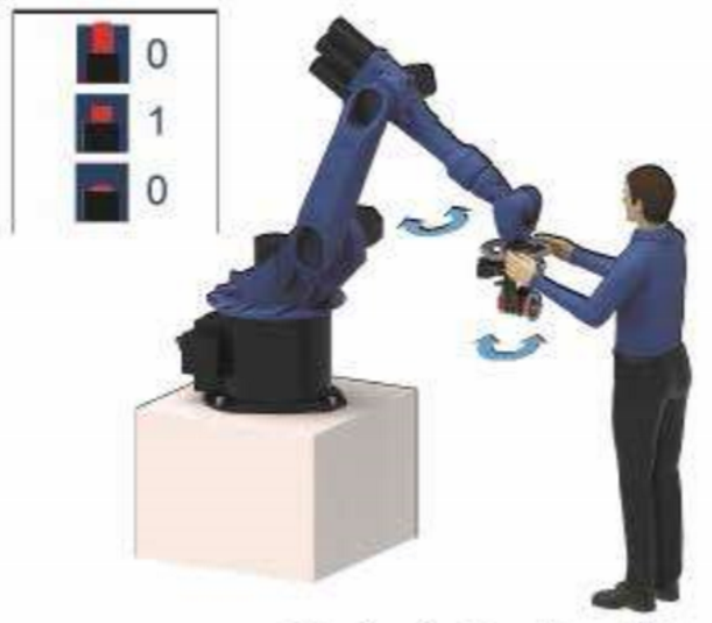
\includegraphics[width=\linewidth]{./bilder/SchutzMRKm2}
    \end{minipage}
\end{minipage}
\clearpage

\begin{minipage}{\linewidth}
    \subsubsection{Geschwindigkeits und Abstandsüberwachung}
    \begin{minipage}{0.7\linewidth}
    \textbf{Methode 3}\newline
    \begin{tabular}{p{2.2cm} p{10cm}}
        \textbf{Prinzip}&
        Kontakt zwischen Mitarbeiter und in Bewegung befindenden Roboter wird vom Roboter vermieden.
        \\
        \textbf{Betriebsweise}&
        Roboter und Bedienperson dürfen sich Gleichzeitig im Kollaborationsraum aufhalten. Es gilt ein Sicherheitsabstand. Wenn das Robotersystem seine Geschwindigkeit herabsetzt, verringert sich auch der Sicherheitsabstand.
        \\
        \textbf{Anwendungs- bereich}&
        Gemeinsame Montage und Handhabung
        \\
    \end{tabular}
    \end{minipage}
    \begin{minipage}{0.3\linewidth}
    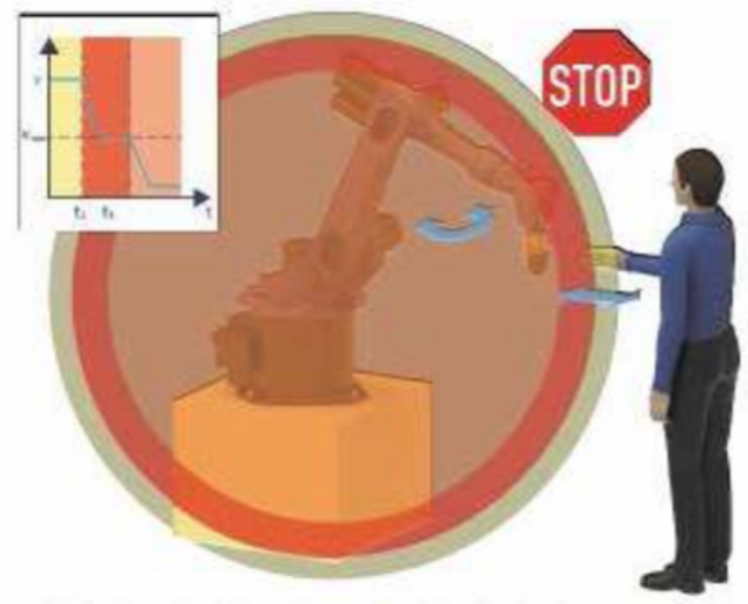
\includegraphics[width=\linewidth]{./bilder/SchutzMRKm3}
    \end{minipage}
\end{minipage}
\begin{minipage}{\linewidth}
    \subsubsection{Leistung und Kraftbegrenzung}
    \begin{minipage}{0.7\linewidth}
    \textbf{Methode 4}\newline
    \begin{tabular}{p{2.2cm} p{10cm}}
        \textbf{Prinzip}&
        Kontaktkräfte zwischen Mitarbeiter unf Roboter(inkl. Bauteil) werden technisch auf ein ungefährliches Mass begrenzt.
        \\
        \textbf{Betriebsweise}&
        Physischer Kontakt zwischen Robotersystem kann auftreten. Jedoch ist die maximale Kraft unterhalb der Belastungsgrenze welche bei der Risikobeurteilung bestimmt wurde.
        \\
        \textbf{Anwendungs- bereich}&
        Kontakt erforderlich(small part assembly)\newline
        Anwendungen, die häufig den Kontakt des Bedienpersonals erfordern
        \\
    \end{tabular}
    \end{minipage}
    \begin{minipage}{0.3\linewidth}
    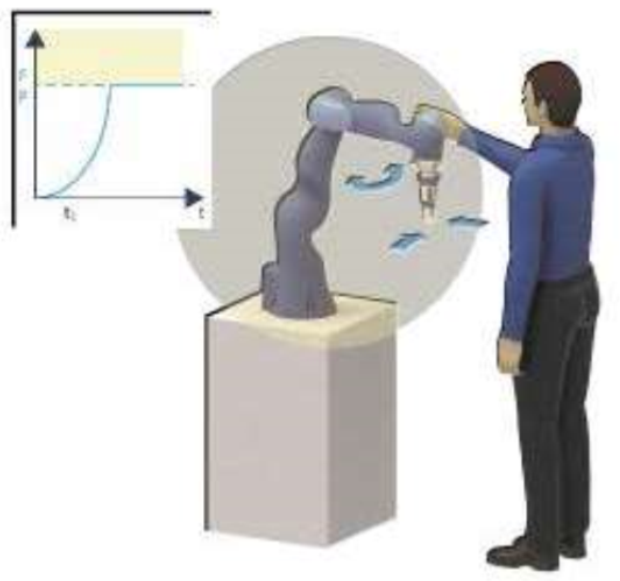
\includegraphics[width=\linewidth]{./bilder/SchutzMRKm4}
    \end{minipage}
\end{minipage}

\subsection{MRK-Arten}
\begin{minipage}[t]{\linewidth}
\begin{minipage}[t]{0.33\linewidth}
\textbf{Koexistenz}\hfill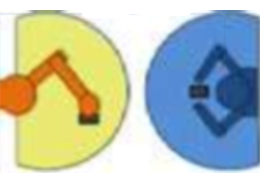
\includegraphics[height=1cm]{./bilder/MRKarten1}
    \begin{itemize}
         \item Getrennter Abreitsbereich
         \item trennende Schutzeinrichtung
    \end{itemize}
\end{minipage}
\begin{minipage}[t]{0.33\linewidth}
    \textbf{Kooperation}\hfill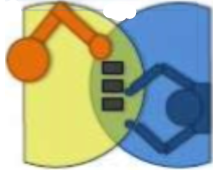
\includegraphics[height=1cm]{./bilder/MRKarten2}
    \begin{itemize}
        \item Externe Sensorik und Sicherheitssteuerung
        \item keine Trenneinrichtung
    \end{itemize}
\end{minipage}
\begin{minipage}[t]{0.33\linewidth}
    \textbf{Kollaboration}\hfill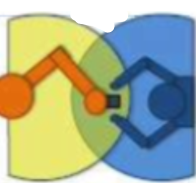
\includegraphics[height=1cm]{./bilder/MRKarten3}
    \begin{itemize}
        \item Integration Sensortechnik zur Leistungs und Kraftbegrenzung
        \item Begrenzung von Kraf bei Kollision
    \end{itemize}
\end{minipage}
\end{minipage}
\begin{tabular}{lll}
    \multirow{2}{3cm}{\textbf{MRK}}&\textbf{Unterschidliche}&\textbf{Gleiche}\\
                &\textbf{Arbeitsräume}&\textbf{Arbeitsräume}\\ \hline
    Sequentielle Bearbeitung& Keine Interaktion& Kooperation\\
    Gleichzeitige Bearbeitung & Koexistenz& Kollaboration\\
\end{tabular}

\subsection{Arten der Kooperation}
\begin{minipage}{0.5\linewidth}
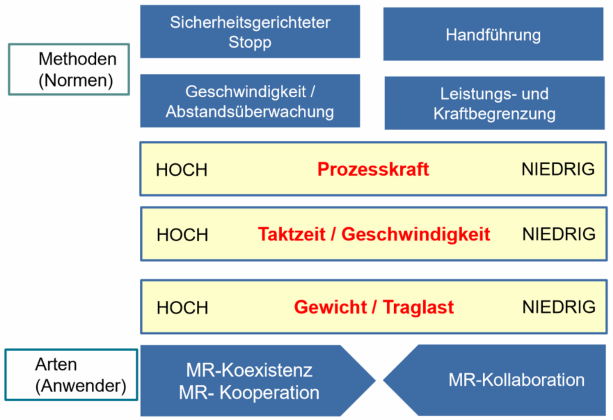
\includegraphics[width=0.8\linewidth]{./bilder/ArtenKooperation}
\end{minipage}
\begin{minipage}{0.5\linewidth}
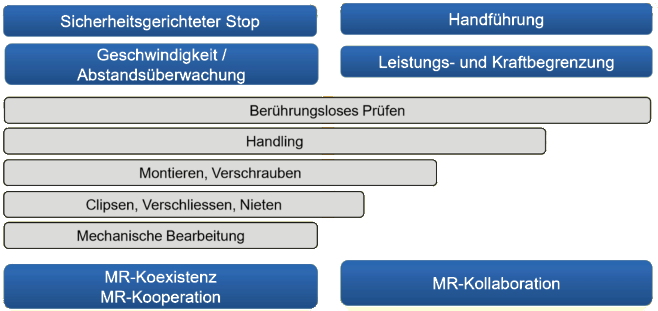
\includegraphics[width=\linewidth]{./bilder/ArtenAnwendungen}
\end{minipage}
\subsection{Kritische Rahmen- / Randbedingungen}
\begin{minipage}{0.5\linewidth}
    \subsubsection{Zykluszeit}
    \begin{itemize}
        \item Sicherheitsbewertete reduzierte Geschwindigkeit 250mm/s
        \item zusätzliche Sicherheitseinrichtung
        \item (In-)Direkte Abhängige Kraft via Geschwindigkeit
        \begin{itemize}
            \item Risikoanalyse, Distanz, Nutzlast, bewegte Robotermasse, Geschwindigkeit
        \end{itemize}
        \item Produktionssteigerung durch Erhöhung der Verfahrensgeschwindigkeit nachträglich möglich
    \end{itemize}
\end{minipage}
\begin{minipage}{0.5\linewidth}
    \subsubsection{Nutzlast/Werkstück}
    \begin{itemize}
        \item hat direkten Einfluss auf bewegte Robotermasse
        \item Direkte Abhängigkeit mit Kraft
        \begin{itemize}
            \item Risikoanalyse, Distanz, Nutzlast, bewegte Robotermasse, Geschwindigkeit
        \end{itemize}
        \item Die grösse kann einfluss auf die Distanz: Handflansch - Schwerpunkt haben
        \item Werkstück-Beschaffenheit wichtig $\rightarrow$ keine scharfen Kanten
    \end{itemize}
\end{minipage}
\begin{minipage}{0.5\linewidth}
    \subsubsection{Arbeistraum/ Interaktion}
    \begin{itemize}
        \item MRK Applikation kann jederzeit durch Kontakt/Eindringen in AR unterbrochen werden
        \item Prozess muss damit umgehen können $\rightarrow$ Reaktion programmieren
        \item Interaktion mit Menschen so eindeutig wie möglich
    \end{itemize}
\end{minipage}
\begin{minipage}{0.5\linewidth}
    \subsubsection{Mehrfacheinsatz}
    \begin{itemize}
        \item Fehlen fester Schutzeinrichtung und "`leichte"' Roboter machen Mehrfacheinsätze interessant
        \item Risikobeurteilung und -management bei (Wieder-)Inbetriebnahme, speziell der Sicherheitseinrichtung, sehr wichtig
    \end{itemize}
\end{minipage}
\subsubsection{Sicherheitsanforderungen}
\begin{itemize}
    \item Es kann zu Kontakt zwischen Roboter und Menschen kommen $\rightarrow$ Sicherheit muss gewährleistet sein
    \item Je nach Methode unterschiedliche Normen
    \item Auf die Sicherheitsanforderung kann einfluss genommen werden durch:
    \begin{itemize}
        \item Applikatio ohne Quetsch- und Druckpunkte
        \item Reduktion der Masse der bewegten Roboterteile
        \item Reduktion der Geschwindigkeit
        \item Veränderung der Roobotergestaltung $\rightarrow$ Vergrösserung der Kontaktfläche
        \item Vermeidung von Kontakt mit sensiblen Körperregionen
    \end{itemize}
\end{itemize}


